\section{RISC-V GPGPU Vortex}

Vortex\footnote{\url{https://github.com/vortexgpgpu/vortex}}~\cite{10.1145/3466752.3480128} is an open-source RISC‑V‑based GPGPU.
It supports OpenCL programming via the POCL compiler\footnote{Portable Computing Language project: \url{https://portablecl.org/}}~\cite{10.1007/s10766-014-0320-y}.
Additionally, it is designed for FPGAs equipped with high-bandwidth memory (HBM), which is advantageous for graph processing.


The high-level architecture of the Vortex processor\footnote{Detailed architectural information is available at \url{https://github.com/vortexgpgpu/vortex/blob/master/docs/microarchitecture.md}.} is shown in Fig.~\ref{fig:vortex_arch}. 
The processor consists of \emph{clusters}, which may share an optional $L_3$ cache.
Each \emph{cluster} contains multiple \emph{sockets}, which may share an optional $L_2$ cache.
\emph{Sockets} consist of cores with shared $L_1$ cache, and each core hosts multiple threads.
Threads share local memory and are logically grouped into warps.

\begin{figure*}
    \begin{center}
        \includegraphics[width=0.8\textwidth]{pictures/Vortex_arch.pdf}
        \caption{Vortex architecture}
        \label{fig:vortex_arch}
    \end{center}
\end{figure*}

The design is flexibly configurable: the numbers of clusters, cores, threads, and warps in the target processor can be specified, and the $L_3$ and $L_2$ caches can be independently enabled or disabled.
Number of sockets calculated automatically such that socket size is a minimum of 4 and number of cores.

The Vortex design is distributed with SimX, a cycle-approximate functional simulator.
A cycle-accurate RTL simulation is also available.
Although the A extension (atomics instructions)\footnote{Supported RISC-V profiles are RV32IMAF and RV64IMAFD (\url{https://github.com/vortexgpgpu/vortex?tab=readme-ov-file\#specifications})} is declared, atomic operations are currently supported only in the SimX simulator and not in the RTL implementation.
